%\begin{enumerate}[label=\thesection.\arabic*.,ref=\thesection.\theenumi]
%\numberwithin{equation}{enumi}

\item

For a control system in unity feedback with a transfer function
\begin{align}
    G(s) = \frac{10K}{s(s+1)(s+5)}
\end{align}
Design a lead compensator with a $60^{\degree}$ phase margin and an appropriate error constant of 5

%\item
\solution
Before adding a compensator, we first find a value of gain for an error constant of 5. As the system has one pole at the origin, the appropriate error constant would be the velocity constant $K_{v}$. For an error constant of 5, we solve the following equation:
\begin{align}
    \lim_{s \to 0} s G(s) = \lim_{s \to 0} \frac{10K}{(s+1)(s+5)} = 2K\\
    \implies K = \frac{K_{v}}{2} = 2.5
\end{align}
So, the new transfer function becomes
\begin{align}
    G(s) = \frac{25}{s(s+1)(s+5)}
\end{align}
The gain crossover frequency $ \omega_{gc} $ and phase margin $ \phi_{M} $ is calculated from the plots using the following code
\begin{lstlisting}
codes/ee18btech11051/ee18btech11051_code1.py
\end{lstlisting}

\begin{figure}[!h]
    \centering
    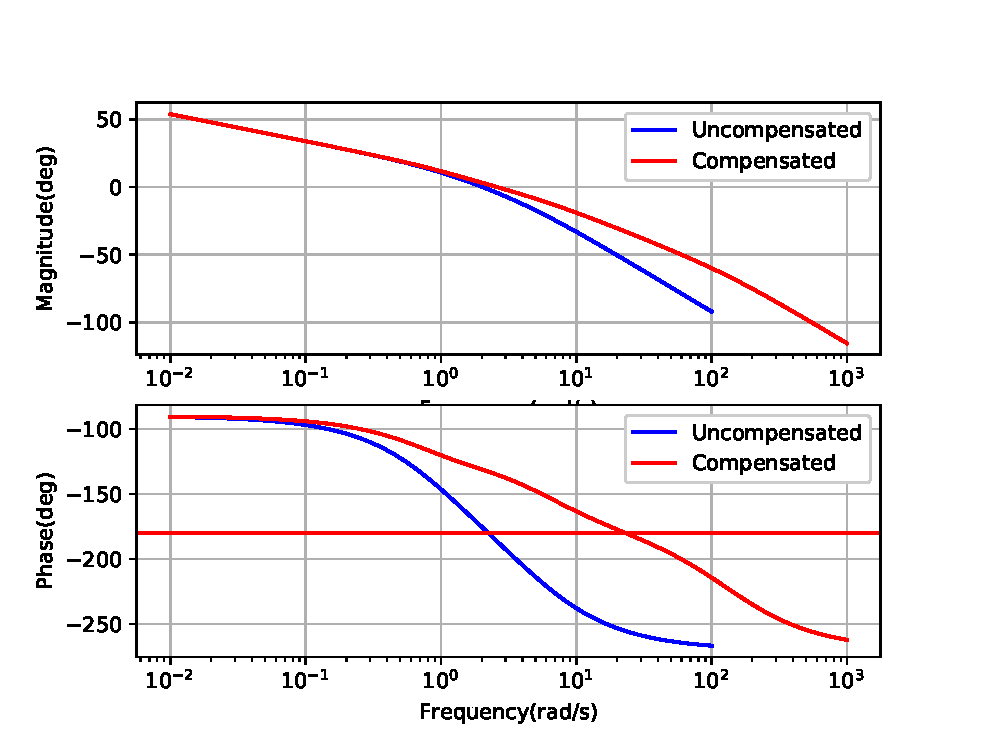
\includegraphics[width=\columnwidth]{./figs/ee18btech11051/ee18btech11051_fig1.eps}
    \label{fig:ee18btech11051_1}
\end{figure}

This can also be calculated from the equations
\begin{align}
    \omega \sqrt{\omega^2 + 1} \sqrt{\omega^2 + 25} = 25\\
    \phi_{M} = -90^{\circ} - \tan^{-1}{\omega_{gc}} - \tan^{-1}({\frac{\omega_{gc}}{10}})
\end{align}
Solving which, we get $\phi_{M} =  3.96^{\degree} , \omega_{gc} =  2.03$\\

The following code computes the margins and frequencies:
\begin{lstlisting}
codes/ee18btech11051/ee18btech11051_code2.py
\end{lstlisting}

The maximum phase of the compensator is given by-
\begin{align}
    \phi_{M} = 60^{\degree} - phase margin + angle correction\\
    \phi_{M} = 56^{\degree} + angle correction
\end{align}
Here, the angle correction is added to compensate the early zero added due to the lead compensator. We set the angle correction to be $20^{\degree}$.
The phase lead compensator will have a transfer function of the form:
\begin{align}
    G_{C}(s) = \left(\frac{1+\alpha Ts} {1+Ts}\right), \alpha >1
\end{align}


Note that this transfer function doesn't change the error constant.
Now we solve for $\alpha$ using the equation
\begin{align}
    \alpha = \frac{1+\sin{\phi_{M}}}{1-\sin{\phi_{M}}} = \frac{1+\sin{76^{\degree}}}{1-\sin{76^{\degree}}} = 66.33
\end{align}

Now to get the phase gain, we set the frequency for maximum phase of compensator $\omega_{m}$ to the previous gain crossover frequency. And using it, the value of T is calculated as follows
\begin{align}
    \omega_{m} = 2.03 rad/sec \\
    T = \frac{1}{\omega_{m}\alpha} = 0.0074
\end{align}


The Compensator will have the transfer function as follows :
\begin{align}
G_{c}(s) = \left(\frac{1 + 0.5s}{1 + 0.0074s}\right)
\end{align}

The open loop T.F for the compensated system is  :
\begin{align}
    G(s) G_{c}(s) = 25\left(\frac{(1+0.5s)}{s(s+1)(s+5)(1+0.0074s)}\right)
\end{align}


%\item
\textbf{Verification : }
To observe the changes, we plot the compensated system

\begin{figure}[!h]
    \centering
    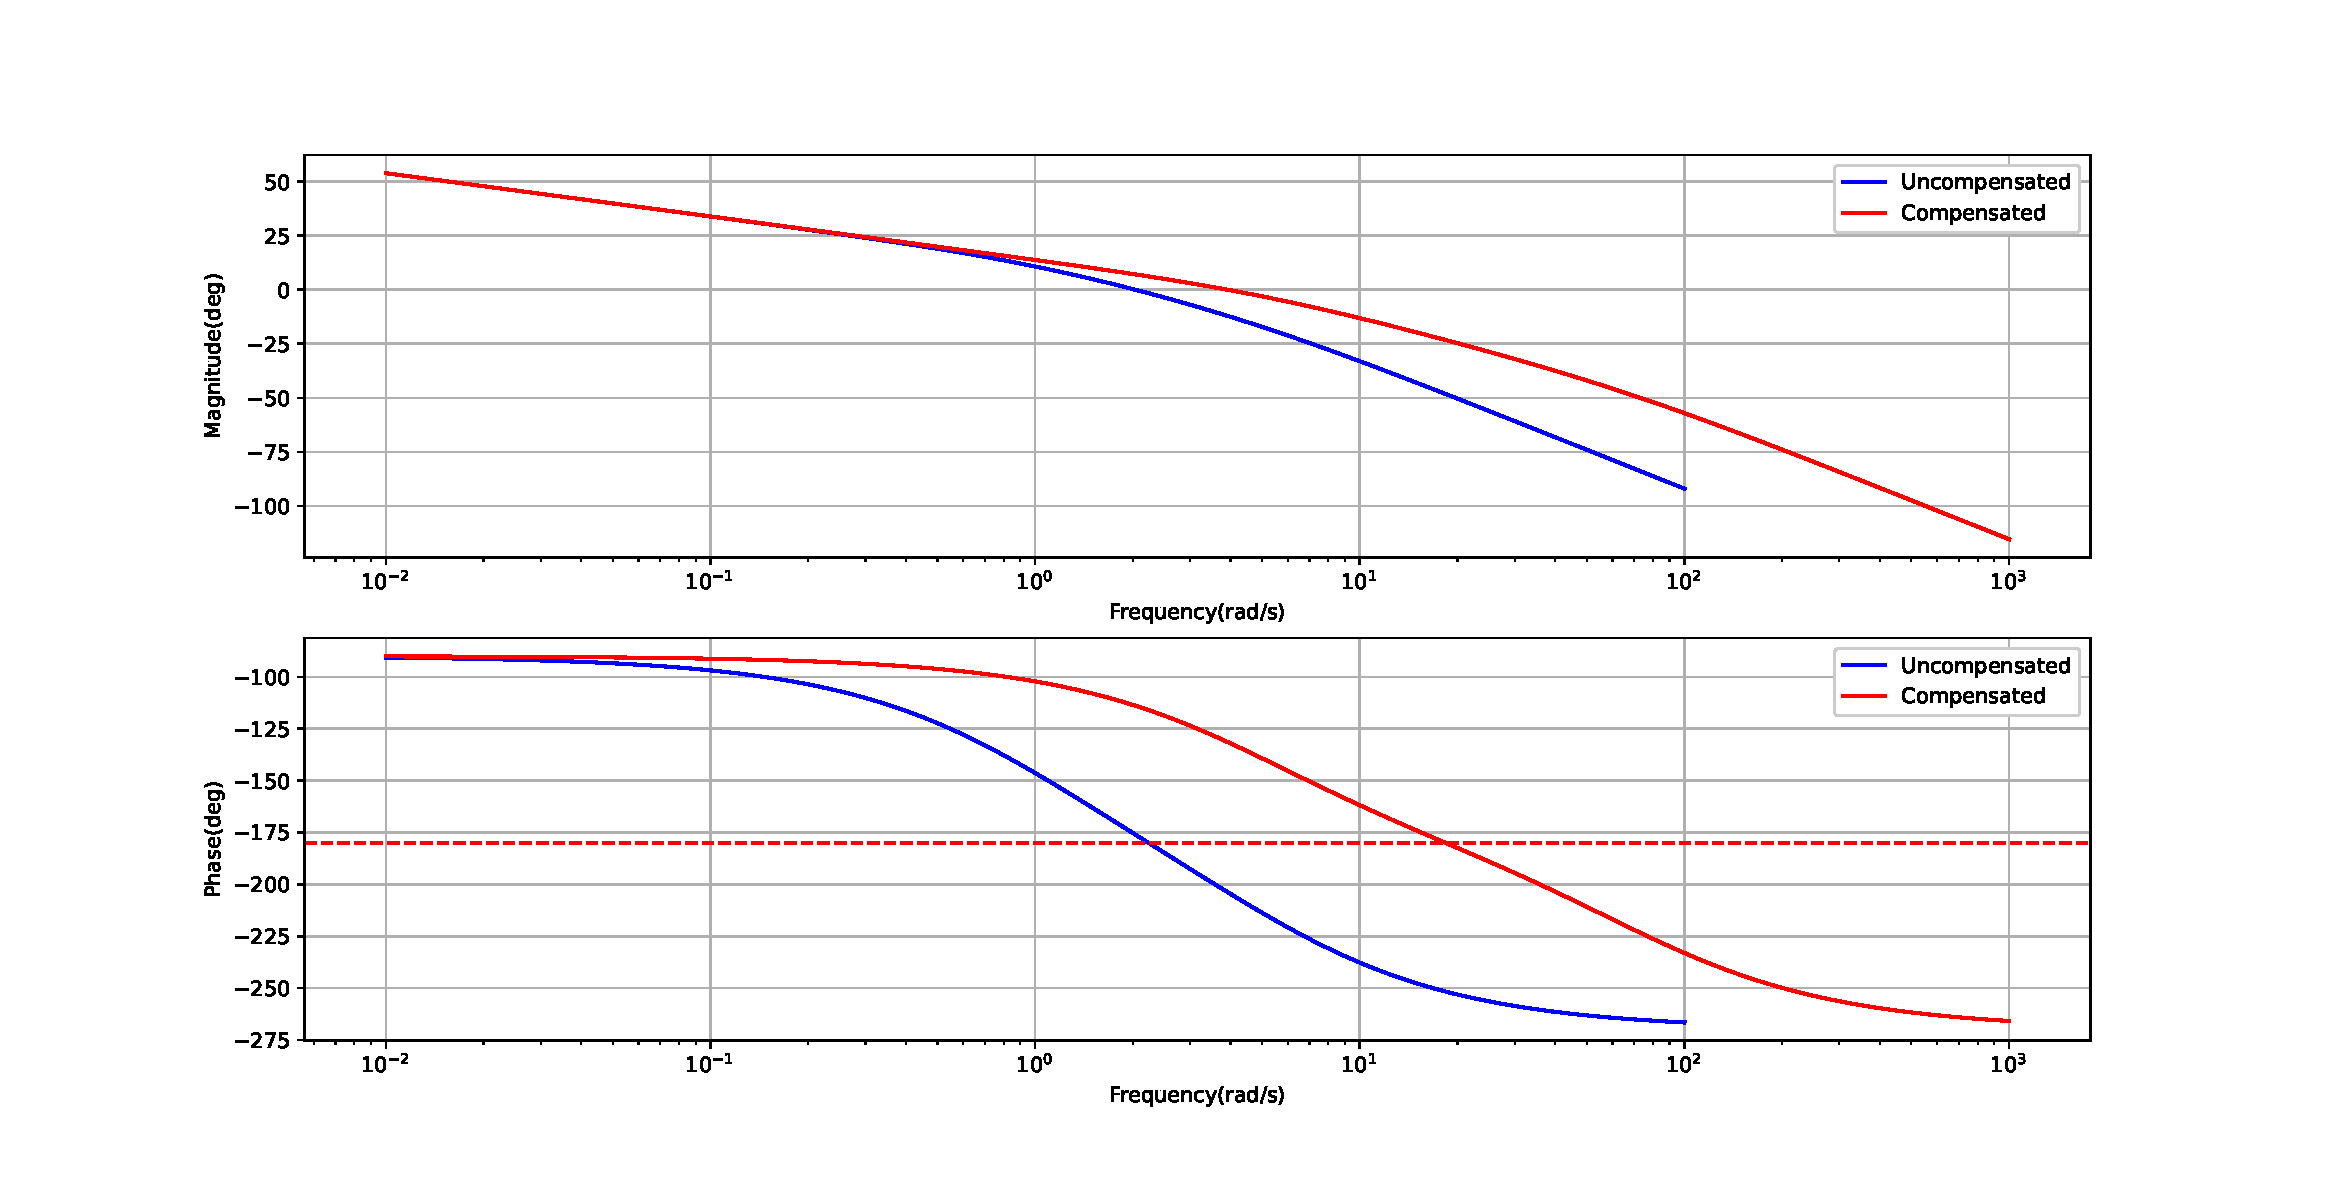
\includegraphics[width=\columnwidth]{./figs/ee18btech11051/ee18btech11051_fig2.eps}
    \label{fig:ee18btech11051_2}
\end{figure}
 Clearly, the gain crossover frequency is slightly shifted to the right due to addition of the early zero, and an overall increase in phase is observed.

%\end{enumerate}
